\documentclass[runningheads,a4paper]{llncs}

\usepackage[portuguese]{babel}
\usepackage[utf8]{inputenc}
\usepackage{amsmath,amssymb}
\setcounter{tocdepth}{3}
\usepackage{graphicx}
\usepackage{url}
\usepackage{indentfirst}


\begin{document}

\mainmatter  % start of an individual contribution

\title{Kropki}
\subtitle{Resolução de Problema de Decisão usando
Programação em Lógica com Restrições}

\author{João Filipe Moreira, Rui Osório}

\institute{Faculdade de Engenharia da Universidade do Porto\\
Rua Roberto Frias, sn, 4200-465 Porto, Portugal\\}

\toctitle{Kropki}
\maketitle

\begin{abstract}
O objetivo deste projeto é fornecer uma solução para o jogo Kropki, um jogo que consiste em um problema de decisão. Para tal é utilizado a Programação Lógica com Restrições, partindo da utilização de Prolog em SicsTus. No final, obteve-se um programa não só capaz de resolver problemas, mas também de os gerar de forma aleatória.
\keywords{kropki, prolog, feup, plr}
\end{abstract}


\section{Introdução}

No âmbito da unidade curricular de Programação em Lógica foi necessário escolher um problema de decisão ou otimização em Prolog para desenvolver as capacidades com restrições, pelo qual acabamos por escolher o Kropki dentro da gama de opções disponibilizada.

O Kropki é um puzzle da família do Sudoku, sendo que neste é necessário preencher todas as células de forma a ter colunas e linhas com números diferentes a partir de umas restrições entre as células.

O artigo aborda uma descrição mais completa do problema, como ele foi modelado em variáveis de decisão e parâmetros, as restrições; a geração aleatória, a visualização da resposta ao problema, os resultados obtidos e a conclusão geral do projeto.

\section{Descrição do Problema}

O puzzle Kropki pertence à família do Sudoku, com uma grelha de tamanho N, onde em cada célula existirão números e com alguns pontos circulares pretos ou brancos na fronteira entre duas células vizinhas.

O ponto preto representa que os valores vizinhos devem ser consecutivos, isto é, possuem uma diferença numérica de 1, e.g. 5 e 6.
O ponto branco representa que um dos valores deve ser o dobro do outro, isto é, multiplicidade de dois, e.g., 2 e 4.

Estes pontos são dados à partida e por isso a falta de pontos entre células vizinhas significa que não existe nenhuma regra de sucessão ou de multiplicidade de 2 que devam obedecer. Para além dos pontos é possível que na configuração inicial sejam já dados alguns valores em algumas células.

\begin{figure}
\centering
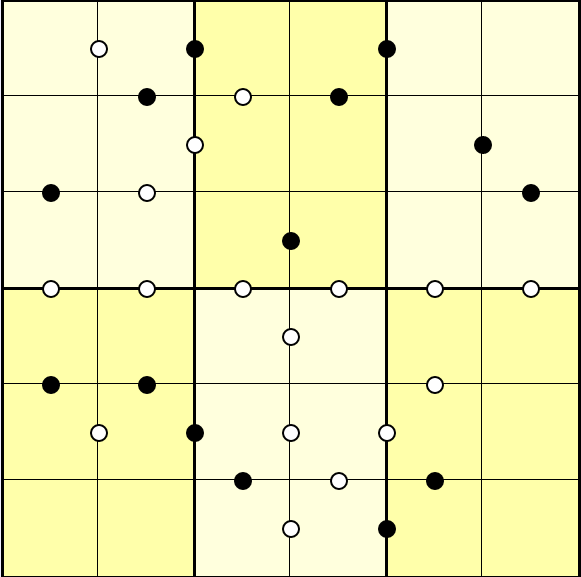
\includegraphics[height=5cm]{res/emptyGrid}
\caption{Grelha num estado inicial}
\label{fig:emptyGrid}
\end{figure}

A finalidade do puzzle é preencher as células vazias pelo qual tem que respeitar as seguintes regras, admitindo um puzzle de dimensão NxN:
\begin{itemize}
  \item Cada célula contém um valor e um valor apenas;
  \item Cada célula contém um número entre 1 e N;
  \item Cada linha não deve ter valores repetidos, ou seja, deve possuir todos os valores de 1 a N uma vez e uma vez apenas;
  \item Cada coluna não deve ter valores repetidos, ou seja, deve possuir todos os valores de 1 a N uma vez e uma vez apenas;
  \item As imposições nas fronteiras devem ser respeitadas.
  \item Entre 1 e 2 tanto pode estar um ponto preto como branco (2 é a sucessão de 1 e 1 multiplicado por 2 é igual a 2.
\end{itemize}

\begin{figure}
\centering
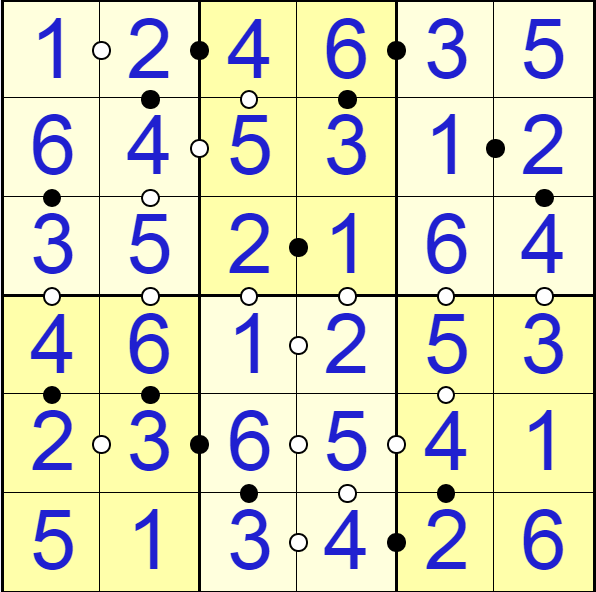
\includegraphics[height=5cm]{res/filledGrid}
\caption{Solução da grelha para o puzzle da figura anterior}
\label{fig:filledGrid}
\end{figure}

\section{Abordagem}

A representação da informação do jogo é feita em grelha, onde nas células são colocados números e nas fronteiras entre as células podem ser colocados pontos ou então estarem vazios.
Nesse sentido, a informação encontra-se na forma matricial que se traduz idealmente em listas de listas em Prolog.

Numa grelha de tamanho \textit{N} temos uma lista de tamanho \textit{N} onde cada item representa uma linha da grelha, sendo que esta é representada também por uma lista que contém \textit{N} valores que correspondem ao número existente na célula, cuja coluna é dada pela posição na lista interna.
Para a informação dos pontos nas fronteiras é utilizada uma estratégia semelhante em que se associa a cada célula um valor que representa o conteúdo da fronteira inferior e à direita.

\subsection{Variáveis de Decisão e Parâmetros}

Para resolver o problema é preciso preencher as células da grelha com números respeitando a configuração proposta e as regras que daí advém.
A configuração do problema consiste no estado da grelha antes de o problema ser abordado e cujos valores são imutáveis durante a resolução. Os pontos e eventuais números nas células são assim os parâmetros.
Para a \textit{BorderList} (lista com os pontos), é garantido que o tamanho da Lista é o correto.

\begin{verbatim}length(BorderList,SizeN)\end{verbatim}

Os números das células advém de \texit{NumberList}, que estará apenas com variáveis se não houver qualquer configuração de número das células. Essas variáveis são colocadas numa só lista através um predicado \textit{joinAll} que pega na lista de listas. 
\begin{verbatim}joinAll(NumberList,JoinedList)\end{verbatim} 
Por fim é necessário garantir que as variáveis estão dentro dos limites impostos, sendo N o tamanho da grelha, é preciso garantir que estarão compreendidos entre 1 e N.

\begin{verbatim}domain(JoinedList,1,SizeN)\end{verbatim}

\subsection{Restrições}

Na grelha é necessário que em cada linha e em cada coluna não exista números repetidos. Para tal existem dois predicados, um que trata das linhas, \textit{mapLine}, e outro que trata das colunas \textit{mapRow}, sendo que ambos utilizam \textit{all\_distinct} após recolherem para uma lista a respetiva linha ou coluna.

\begin{verbatim}mapLine(NumberList)\end{verbatim}
\begin{verbatim}mapRow(NumberList)\end{verbatim}

Contudo a última tem que fazer um implementação mais complexa, visto necessitar de ir a cada linha buscar o valor da coluna que é necessário processar antes de juntar a uma lista, ao contrário da primeira que pode ir retirar a linha imediatamente da lista de listas.
Assegurado que as duas condições anteriores é necessário que as restrições impostas pelos pontos também se verifiquem, logo tem-se:

\begin{verbatim}cycle(NumberList,BorderList)\end{verbatim}


Este predicado vai a cada célula e pega no elemento dessa célula e na informação de fronteira (direita e em baixo) e verifica se existe alguma restrição que se enquadra. Se essa célula não tiver qualquer informação:

\begin{verbatim}restriction(_,_,_,_,0)\end{verbatim}

Se por exemplo nessa célula houver um ponto branco (números sucessivos) à direita, é calculado a posição da coluna à direita para obter o valor dessa célula e na última instrução é estabelecida a restrição:

\begin{verbatim}
restriction(NumberList,NumberElement,PosX,PosY,1):-tabSize(Nsize),
PosYnew is PosY +1,
PosYnew<Nsize,
nth0(PosX,NumberList,Line),
nth0(PosYnew,Line,NextColElement),!,
NumberElement#=NextColElement+1#\/NumberElement#=NextColElement-1.
\end{verbatim}

Se houver um ponto preto, a situação é semelhante só que o cabeçalho e última instrução serão:
\begin{verbatim}
restriction(NumberList,NumberElement,PosX,PosY,2)
...
NumberElement#=NextColElement*2#\/NextColElement#=NumberElement*2.
\end{verbatim}

\section{Visualização da Solução}

\section{Resultados}

\section{Conclusões}

Após a realização deste trabalho é possível extrapolar a preferência na utilização do Prolog para problemas como a resolução de puzzles uma vez que sendo uma linguagem lógica permite, com maior facilidade do que outras linguagens, definir regras de puzzles. É também com confiança que se afirma que o programa desenvolvido é capaz de resolver uma considerável parte dos puzzles do tipo Kropki em tempos aceitáveis (menos que 2 segundos), baseando tal afirmação na rapidez com que o programa resolveu os tabuleiros de teste até ao tamanho 8x8 e de se ter constatado que a considerável parte dos desafios do puzzle Kropki encontrados não possuem dimensões superiores a 7x7.

No entanto, seria desejável encontrar uma maneira de realizar uma pré-análise que determinasse quão eficaz o programa seria a resolver o puzzle em questão. Por conseguinte seria possível fornecer mais informação ao utilizador sobre a probabilidade de obter uma resolução, fazendo com que este não fique refém de uma resolução que poderá nunca ser obtida.

\begin{thebibliography}{4}

\bibitem{url} Star Battle rules,\\
\url{http://logicmastersindia.com/lmitests/dl.asp?attachmentid=430}

\bibitem{url} SICStus Prolog, \url{https://sicstus.sics.se/}

\bibitem{url} SWI-Prolog, \url{http://www.swi-prolog.org/}

\end{thebibliography}

\pagebreak

\section*{Anexo}

\subsection*{Código fonte}

\newenvironment{changemargin}[2]{%
\begin{list}{}{%
\setlength{\topsep}{0pt}%
\setlength{\leftmargin}{#1}%
\setlength{\rightmargin}{#2}%
\setlength{\listparindent}{\parindent}%
\setlength{\itemindent}{\parindent}%
\setlength{\parsep}{\parskip}%
}%
\item[]}{
\end{list}}

\medskip

\noindent
{\it starBattle.pl}
\begin{changemargin}{-3cm}{-4cm}
\begin{verbatim}

%=============================================%
%=                                           =%
%=           ..:: STAR BATTLE ::..           =%
%=                                           =%
%=        Type 'starBattle.' to start        =%
%=                                           =%
%=============================================%
%=                                           =%
%=             ..:: Authors ::..             =%
%=                                           =%
%=     Henrique Ferrolho && Joao Pereira     =%
%=                FEUP - 2014                =%
%=                                           =%
%=============================================%

%===============%
%= @@ includes =%
%===============%
:- use_module(library(clpfd)).
:- include('containers.pl').
:- include('printer.pl').
:- include('solver.pl').
:- include('starBattleTestBoards.pl').
:- include('utilities.pl').

%====================%
%= @@ game launcher =%
%====================%
starBattle:-
    clearConsole,
    write('To run the program type:'), nl,
    nl,
    write('\tstarBattle(NumBoard, NumStars).'),nl,
    nl,
    write('- NumBoard'), nl,
    write('number of the board you wish to test.'), nl,
    nl,
    write('- NumStars'), nl,
    write('number of stars you wish to place on each row, column and region.'), nl,
    nl.

starBattle(BoardNumber, NumStars):-
    clearConsole,
    write('==============='), nl,
    write('= Star Battle ='), nl,
    write('==============='), nl,
    nl,
    format('Trying to place ~d stars on board no. ~d:', [NumStars, BoardNumber]), nl,

    getBoard(BoardNumber, Board),
    printBoard(Board), !,

    solveBoard(Board, NumStars, Result), !,
    pressEnterToContinue,

    %getBoardSize(Board, BoardSize),
    %printResult(Result, BoardSize, NumStars),
    printResultBoard(Board, Result, NumStars), !.
    
    
\end{verbatim}
\end{changemargin}

\noindent
{\it solver.pl}
\begin{changemargin}{-3cm}{-4cm}
\begin{verbatim}

solveBoard(Board, S, Result):-
    getBoardSize(Board, N),

    % a board NxN can not have more than N/2 stars
    S #=< (N - 1) // 2 + 1,

    ResultLength #= N * S,

    length(Result, ResultLength),
    length(ResultRegions, ResultLength),

    domain(Result, 1, N),
    domain(ResultRegions, 1, N),

    % 1st restriction
    validateNumOfOccurrencesForEachElem(Result, S, N),

    % 2nd restriction
    fetchResultRegions(Board, Result, N, S, ResultRegions),
    validateNumOfOccurrencesForEachElem(ResultRegions, S, N),

    % 3rd restriction
    noAdjacentStars(Result, S, N),

    statistics(walltime, _),
    labeling([bisect], Result),
    statistics(walltime, [_, ElapsedTime | _]),
    format('An answer has been found!~nElapsed time: ~3d seconds', ElapsedTime), nl,
    fd_statistics,
    nl.


%-%-%-%-%-%-%-%-%-%-%-%-%-%-%-%-%-%-%-%-%-%-%-%-%-%-%-%-%-%-%-%-%-%-%

getBoardSize([Head|_], N):-
    length(Head, N).


%-%-%-%-%-%-%-%-%-%-%-%-%-%-%-%-%-%-%-%-%-%-%-%-%-%-%-%-%-%-%-%-%-%-%

validateNumOfOccurrencesForEachElem(Elements, NumOfOccurrences, N):-
    validateNumOfOccurrencesForEachElem(Elements, NumOfOccurrences, N, 1).

validateNumOfOccurrencesForEachElem(Result, S, N, N):-
    exactly(N, Result, S).
validateNumOfOccurrencesForEachElem(Result, S, N, I):-
    exactly(I, Result, S),
    I1 #= I + 1,
    validateNumOfOccurrencesForEachElem(Result, S, N, I1).


%-%-%-%-%-%-%-%-%-%-%-%-%-%-%-%-%-%-%-%-%-%-%-%-%-%-%-%-%-%-%-%-%-%-%

fetchResultRegions(Board, Result, ResRows, ResCols, ResultRegions):-
    fetchResultRegions(Board, Result, ResRows, ResCols, [], 1, ResultRegions).

fetchResultRegions(_, _, ResRows, ResCols, ResultRegions, Pos, ResultRegions):-
    Pos #= ResRows * ResCols + 1.
fetchResultRegions(Board, Result, ResRows, ResCols, ResultRegionsSoFar, Pos, ResultRegions):-
    % calculating row and col of result to access
    Row #= (Pos - 1) // ResCols + 1,
    Col #= ((Pos - 1) mod ResCols) + 1,

    % get the value of result[Row][Col], which is the column where a star is placed
    getMatrixOfListElemAt(Result, ResRows, ResCols, Row, Col, StarCol),

    % get line Row of the board
    getListElemAt(Board, Row, Line),

    % get the region of that position - board[Row][StarCol]
    element(StarCol, Line, Region),

    % push value to ResultRegionsSoFar
    listPushBack(ResultRegionsSoFar, Region, NewResultRegionsSoFar),

    % fetch next element
    Pos1 #= Pos + 1,
    fetchResultRegions(Board, Result, ResRows, ResCols, NewResultRegionsSoFar, Pos1, ResultRegions).


%-%-%-%-%-%-%-%-%-%-%-%-%-%-%-%-%-%-%-%-%-%-%-%-%-%-%-%-%-%-%-%-%-%-%

noAdjacentStars(Result, S, N):-
    noAdjacentStars(Result, S, N, 1).

noAdjacentStars(Result, S, N, 1):-
    noAdjacentStarsOnRow(Result, S, 1),
    noAdjacentStars(Result, S, N, 2).
noAdjacentStars(_, _, N, Row):-
    Row #= N + 1.
noAdjacentStars(Result, S, N, Row):-
    Row #> 1,
    noAdjacentStarsOnRow(Result, S, Row),
    noAdjacentStarsWithPreviousRow(Result, S, Row),
    Row1 #= Row + 1,
    noAdjacentStars(Result, S, N, Row1).


%-%-%-%-%-%-%-%-%-%-%-%-%-%-%-%-%-%-%-%-%-%-%-%-%-%-%-%-%-%-%-%-%-%-%

noAdjacentStarsOnRow(Result, S, Row):-
    StartPos #= (Row - 1) * S + 1,
    EndPos #= StartPos + S,
    validateStarsFromStartToEnd(Result, StartPos, EndPos).

validateStarsFromStartToEnd(Result, Start, End):-
    Next #= Start + 1,
    validateStarsFromStartToEnd(Result, Start, Next, End).

validateStarsFromStartToEnd(_, Start, _, End):-
    Start #= End - 1.
validateStarsFromStartToEnd(Result, Start, End, End):-
    Start1 #= Start + 1,
    Next #= Start1 + 1,
    validateStarsFromStartToEnd(Result, Start1, Next, End).
validateStarsFromStartToEnd(Result, Start, Next, End):-
    validateHorizontalDistanceBetweenStars(Result, Start, Next),
    Next1 #= Next + 1,
    validateStarsFromStartToEnd(Result, Start, Next1, End).


%-%-%-%-%-%-%-%-%-%-%-%-%-%-%-%-%-%-%-%-%-%-%-%-%-%-%-%-%-%-%-%-%-%-%

noAdjacentStarsWithPreviousRow(Result, S, Row):-
    StartPos #= (Row - 1) * S + 1,
    EndPos #= StartPos + S,
    noAdjacentStarsWithPreviousRow(Result, S, Row, StartPos, EndPos).

noAdjacentStarsWithPreviousRow(_, _, _, EndPos, EndPos).
noAdjacentStarsWithPreviousRow(Result, S, Row, CurrentPos, EndPos):-
    % for each star of the row being validated,
    % validate horizontal distance to each star of the previous row
    PrevRow #= Row - 1,
    starIsNotAdjacentWithAnyOfThePreviousRow(Result, S, CurrentPos, PrevRow),
    % procceed to next row
    CurrentPos1 #= CurrentPos + 1,
    noAdjacentStarsWithPreviousRow(Result, S, Row, CurrentPos1, EndPos).

starIsNotAdjacentWithAnyOfThePreviousRow(Result, S, PivotStar, PrevRow):-
    FirstStarPos #= (PrevRow - 1) * S + 1,
    LastStarPos #= FirstStarPos + S,
    starIsNotAdjacentToAnyOtherStarFromFirstToLastPos(Result, PivotStar, FirstStarPos, LastStarPos).

starIsNotAdjacentToAnyOtherStarFromFirstToLastPos(_, _, LastStarPos, LastStarPos).
starIsNotAdjacentToAnyOtherStarFromFirstToLastPos(Result, PivotStar, CurrentStarPos, LastStarPos):-
    validateHorizontalDistanceBetweenStars(Result, PivotStar, CurrentStarPos),
    NextStarPos #= CurrentStarPos + 1,
    starIsNotAdjacentToAnyOtherStarFromFirstToLastPos(Result, PivotStar, NextStarPos, LastStarPos).


%-%-%-%-%-%-%-%-%-%-%-%-%-%-%-%-%-%-%-%-%-%-%-%-%-%-%-%-%-%-%-%-%-%-%

validateHorizontalDistanceBetweenStars(Result, Pos1, Pos2):-
    element(Pos1, Result, Col1),
    element(Pos2, Result, Col2),
    Dist #= abs(Col2 - Col1),
    Dist #> 1.
    
    
\end{verbatim}
\end{changemargin}

\noindent
{\it printer.pl}
\begin{changemargin}{-3cm}{-4cm}
\begin{verbatim}

%===============================%
%= @@ board printing functions =%
%===============================%
printBoard(Board):-
    getBoardSize(Board, N),
    printBoardTopBorder(N),
    printBoard(Board, 1, N),
    nl, !.
printResultBoard(Board, Result, S):-
    getBoardSize(Board, N),
    printBoardTopBorder(N),
    printBoard(Board, 1, N, Result, S),
    nl, !.

printBoardTopBorder(N):-
    N1 is N - 1, createSeparatorN(N1, '______', TopBorder),
    write(' '), printList(TopBorder), write('_____'), nl.

printBoard(Board, N, N):-
    printBoardRow(Board, N, N).
printBoard(Board, I, N):-
    printBoardRow(Board, I, N), !,
    I1 is I + 1,
    printBoard(Board, I1, N).
%-%-%-%-%-%-%
printBoard(Board, N, N, Result, S):-
    printBoardRow(Board, N, N, Result, S).
printBoard(Board, I, N, Result, S):-
    printBoardRow(Board, I, N, Result, S), !,
    I1 is I + 1,
    printBoard(Board, I1, N, Result, S).

%-%-%-%-%-%-%-%-%-%-%-%-%-%-%-%-%-%-%-%-%-%-%-%-%-%-%-%-%-%-%-%-%-%-%

printBoardRow(Board, N, N):-
    write('|'), printBoardRowTop(Board, N, N, 1), nl, !,
    write('|'), printBoardRowMiddle(Board, N, N, 1), nl, !,
    write('|'), printBoardLastRowBottom(Board, N, N, 1), nl, !.
printBoardRow(Board, I, N):-
    write('|'), printBoardRowTop(Board, I, N, 1), nl, !,
    write('|'), printBoardRowMiddle(Board, I, N, 1), nl, !,
    write('|'), printBoardRowBottom(Board, I, N, 1), nl, !.
%-%-%-%-%-%-%
printBoardRow(Board, N, N, Result, S):-
    write('|'), printBoardRowTop(Board, N, N, 1), nl, !,
    write('|'), printBoardRowMiddle(Board, N, N, 1, Result, S), nl, !,
    write('|'), printBoardLastRowBottom(Board, N, N, 1), nl, !.
printBoardRow(Board, I, N, Result, S):-
    write('|'), printBoardRowTop(Board, I, N, 1), nl, !,
    write('|'), printBoardRowMiddle(Board, I, N, 1, Result, S), nl, !,
    write('|'), printBoardRowBottom(Board, I, N, 1), nl, !.

%-%-%-%-%-%-%-%-%-%-%-%-%-%-%-%-%-%-%-%-%-%-%-%-%-%-%-%-%-%-%-%-%-%-%

printBoardRowTop(_, _, N, N):-
    write('     |').
printBoardRowTop(Board, I, N, Col):-
    getListElemAt(Board, I, Row),
    Col1 is Col + 1,
    element(Col, Row, V1),
    element(Col1, Row, V2),
    printCellTop(V1, V2),
    printBoardRowTop(Board, I, N, Col1).

% @@@ swap comment to toggle region display
%printBoardRowMiddle(Board, I, N, N):-
%   getListElemAt(Board, I, Row),
%   element(N, Row, V1),
%   write('  '), write(V1), write('  |').
printBoardRowMiddle(_, _, N, N):-
    write('     |').
printBoardRowMiddle(Board, I, N, Col):-
    getListElemAt(Board, I, Row),
    Col1 is Col + 1,
    element(Col, Row, V1),
    element(Col1, Row, V2),
    printValue(V1, V2),
    printBoardRowMiddle(Board, I, N, Col1).
%-%-%-%-%-%-%
printBoardRowMiddle(_, I, N, N, Result, S):-
    starExistsIn(Result, S, I, N),
    write('  *  |').
printBoardRowMiddle(_, _, N, N, _, _):-
    write('     |').
printBoardRowMiddle(Board, I, N, Col, Result, S):-
    starExistsIn(Result, S, I, Col),

    getListElemAt(Board, I, Row),
    Col1 is Col + 1,
    element(Col, Row, V1),
    element(Col1, Row, V2),
    printStar(V1, V2),
    printBoardRowMiddle(Board, I, N, Col1, Result, S).
printBoardRowMiddle(Board, I, N, Col, Result, S):-
    getListElemAt(Board, I, Row),
    Col1 is Col + 1,
    element(Col, Row, V1),
    element(Col1, Row, V2),
    printValue(V1, V2),
    printBoardRowMiddle(Board, I, N, Col1, Result, S).

printBoardRowBottom(Board, I, N, N):-
    getListElemAt(Board, I, Row),
    I1 is I + 1, getListElemAt(Board, I1, NextRow),

    element(N, Row, V1),
    element(N, NextRow, V3),

    printCellBottom(V1, V3).
printBoardRowBottom(Board, I, N, Col):-
    getListElemAt(Board, I, Row),
    I1 is I + 1, getListElemAt(Board, I1, NextRow),
    NextCol is Col + 1,

    element(Col, Row, V1),
    element(NextCol, Row, V2),
    element(Col, NextRow, V3),

    printCellBottom(V1, V2, V3),
    printBoardRowBottom(Board, I, N, NextCol).

printBoardLastRowBottom(_, _, N, N):-
    write('_____|').
printBoardLastRowBottom(Board, I, N, Col):-
    getListElemAt(Board, I, Row),
    NextCol is Col + 1,

    element(Col, Row, V1),
    element(NextCol, Row, V2),

    printLastRowCellBottom(V1, V2),
    printBoardLastRowBottom(Board, I, N, NextCol).

%-%-%-%-%-%-%-%-%-%-%-%-%-%-%-%-%-%-%-%-%-%-%-%-%-%-%-%-%-%-%-%-%-%-%

printCellTop(V1, V1):-
    write('     .').
printCellTop(_, _):-
    write('     |').

% @@@ swap comment to toggle region display
%printValue(V, V):-
%   write('  '), write(V), write('  .').
printValue(V, V):-
    write('     .').

% @@@ swap comment to toggle region display
%printValue(V, _):-
%   write('  '), write(V), write('  |').
printValue(_, _):-
    write('     |').

printStar(V, V):-
    write('  *  .').
printStar(_, _):-
    write('  *  |').

printCellBottom(V, V, V):-
    write(' . . .').
printCellBottom(V, V, _):-
    write('_____.').
printCellBottom(V, _, V):-
    write(' . . |').
printCellBottom(_, _, _):-
    write('_____|').

printCellBottom(V, V):-
    write(' . . |').
printCellBottom(_, _):-
    write('_____|').

printLastRowCellBottom(V, V):-
    write('______').
printLastRowCellBottom(_, _):-
    write('_____|').


%-%-%-%-%-%-%-%-%-%-%-%-%-%-%-%-%-%-%-%-%-%-%-%-%-%-%-%-%-%-%-%-%-%-%

createSeparatorN(0, _, []).
createSeparatorN(N, SS, [SS | Ls]):-
    N1 is N-1,
    createSeparatorN(N1, SS, Ls).


%-%-%-%-%-%-%-%-%-%-%-%-%-%-%-%-%-%-%-%-%-%-%-%-%-%-%-%-%-%-%-%-%-%-%

starExistsIn(Result, S, Row, StarCol):-
    StartPos is (Row - 1) * S + 1,
    EndPos is StartPos + S,
    starExistsSomewhereBetween(Result, StartPos, EndPos, StarCol).

starExistsSomewhereBetween(Result, CurrentPos, _, StarCol):-
    element(CurrentPos, Result, ScanRes),
    StarCol =:= ScanRes.
starExistsSomewhereBetween(Result, CurrentPos, EndPos, StarCol):-
    NextPos is CurrentPos + 1,
    NextPos < EndPos,
    starExistsSomewhereBetween(Result, NextPos, EndPos, StarCol).


%================================%
%= @@ result printing functions =%
%================================%
printResult(Result, N, S):-
    write('Result:'), nl,
    printResultRow(Result, N, S, 1).


printResultRow(Result, N, S, N):-
    write('\t'), printResultRowValues(Result, N, S, N, 1).

printResultRow(Result, N, S, Row):-
    write('\t'), printResultRowValues(Result, N, S, Row, 1),

    Row1 is Row + 1,
    printResultRow(Result, N, S, Row1).


printResultRowValues(Result, _, S, Row, S):-
    Pos is (Row - 1) * S + S,
    getListElemAt(Result, Pos, Elem),
    write(Elem), nl.

printResultRowValues(Result, N, S, Row, Column):-
    Pos is (Row - 1) * S + Column,
    getListElemAt(Result, Pos, Elem),
    write(Elem), write(', '),

    Column1 is Column + 1,
    printResultRowValues(Result, N, S, Row, Column1).
    
    
\end{verbatim}
\end{changemargin}

\noindent
{\it containers.pl}
\begin{changemargin}{-3cm}{-4cm}
\begin{verbatim}

%=================%
%= @@ containers =%
%=================%
% containers are indexed starting at 1, not 0.

%%% 1. matrix; 2. element row; 3. element column; 4. query element.
getMatrixElemAt([ListAtTheHead|_], 1, ElemCol, Elem):-
    getListElemAt(ListAtTheHead, ElemCol, Elem).
getMatrixElemAt([_|RemainingLists], ElemRow, ElemCol, Elem):-
    ElemRow > 1,
    ElemRow1 is ElemRow - 1,
    getMatrixElemAt(RemainingLists, ElemRow1, ElemCol, Elem).

% treats list as if it was a matrix of NRows x NCols and returns the Elem at ElemRow, ElemCol
getMatrixOfListElemAt(List, NRows, NCols, ElemRow, ElemCol, Elem):-
    ElemRow =< NRows, ElemCol =< NCols,
    Pos is (ElemRow - 1) * NCols + ElemCol,
    element(Pos, List, Elem).

%%% 1. list; 2. element position; 3. query element.
getListElemAt([ElemAtTheHead|_], 1, ElemAtTheHead).
getListElemAt([_|RemainingElems], Pos, Elem):-
    Pos > 1,
    Pos1 is Pos - 1,
    getListElemAt(RemainingElems, Pos1, Elem).

listPushBack([], Elem, [Elem]).
listPushBack([Head|Tail], Elem, [Head|NewTail]):-
    listPushBack(Tail, Elem, NewTail).

printList([]).
printList([Head|Tail]):-
    write(Head), printList(Tail).
    
    
\end{verbatim}
\end{changemargin}

\noindent
{\it utilities.pl}
\begin{changemargin}{-3cm}{-4cm}
\begin{verbatim}

%================%
%= @@ utilities =%
%================%
clearConsole:-
    clearConsole(40), !.
clearConsole(0).
clearConsole(N):-
    nl,
    N1 is N-1,
    clearConsole(N1).

pressEnterToContinue:-
    write('Press <Enter> to show the solution.'), nl,
    waitForEnter, !.
waitForEnter:-
    get_char(_).

exactly(_, [], 0).
exactly(X, [Y|L], N) :-
    X #= Y #<=> B,
    N #= M + B,
    exactly(X, L, M).
    
    
\end{verbatim}
\end{changemargin}

\noindent
{\it starBattleTestBoards.pl}
\begin{changemargin}{-3cm}{-4cm}
\begin{verbatim}

%=======================================%
%= @@ function to retrieve test boards =%
%=======================================%
getBoard(N, Board):-
    (
        N =:= 1 -> testBoard4x4_1(Board);
        N =:= 2 -> testBoard5x5_1(Board);
        N =:= 3 -> testBoard5x5_2(Board);
        N =:= 4 -> testBoard8x8_1(Board);
        N =:= 5 -> testBoard8x8_2(Board);
        N =:= 6 -> testBoard10x10_1(Board);
        N =:= 7 -> testBoard10x10_2(Board);

        nl,
        write('Error: the specified board does not exist.'),
        fail
    ).

%==================%
%= @@ test boards =%
%==================%
% expected answer:2413
testBoard4x4_1([
    [1, 2, 1, 1],
    [1, 1, 1, 3],
    [4, 1, 1, 1],
    [1, 1, 1, 1]]).

% expected answer: 14253
testBoard5x5_1([
    [1, 1, 2, 2, 2],
    [1, 2, 2, 3, 2],
    [1, 2, 2, 2, 2],
    [4, 2, 4, 2, 5],
    [4, 4, 4, 5, 5]]).

testBoard5x5_2([
    [1, 1, 1, 2, 2],
    [1, 3, 3, 3, 4],
    [1, 1, 3, 3, 4],
    [1, 5, 5, 5, 5],
    [1, 1, 1, 5, 5]]).

% expected answer: 2468246813571357
testBoard8x8_1([
    [1, 2, 3, 4, 5, 6, 7, 8],
    [1, 2, 3, 4, 5, 6, 7, 8],
    [1, 2, 3, 4, 5, 6, 7, 8],
    [1, 2, 3, 4, 5, 6, 7, 8],
    [1, 2, 3, 4, 5, 6, 7, 8],
    [1, 2, 3, 4, 5, 6, 7, 8],
    [1, 2, 3, 4, 5, 6, 7, 8],
    [1, 2, 3, 4, 5, 6, 7, 8]]).

% expected answer: 2468246813571357
testBoard8x8_2([
    [1, 1, 1, 1, 1, 1, 1, 1],
    [2, 2, 2, 2, 2, 2, 2, 2],
    [3, 3, 3, 3, 3, 3, 3, 3],
    [4, 4, 4, 4, 4, 4, 4, 4],
    [5, 5, 5, 5, 5, 5, 5, 5],
    [6, 6, 6, 6, 6, 6, 6, 6],
    [7, 7, 7, 7, 7, 7, 7, 7],
    [8, 8, 8, 8, 8, 8, 8, 8]]).

testBoard10x10_1([
    [1,  1,  1,  2,  2,  3,  3,  3,  3,  3],
    [1,  4,  4,  4,  2,  5,  3,  5,  3,  6],
    [1,  1,  1,  4,  2,  5,  3,  5,  6,  6],
    [1,  4,  4,  4,  2,  5,  5,  5,  6,  6],
    [1,  4,  7,  7,  7,  8,  9,  5,  9,  6],
    [1,  4,  4,  4,  7,  8,  9,  5,  9,  6],
    [1,  1,  7,  7,  7,  8,  9,  9,  9,  6],
    [10, 10, 7,  8,  8,  8,  8,  8,  9,  6],
    [10, 10, 7,  7,  7,  10, 6,  8,  9,  6],
    [10, 10, 10, 10, 10, 10, 6,  6,  6,  6]]).

testBoard10x10_2([
    [1,  1,  1,  2,  2,  2,  2,  2,  2,  2],
    [3,  3,  1,  1,  1,  1,  2,  2,  2,  2],
    [3,  4,  4,  4,  4,  5,  5,  5,  5,  2],
    [3,  4,  4,  4,  4,  5,  5,  5,  6,  2],
    [3,  7,  7,  7,  7,  7,  7,  5,  6,  2],
    [3,  7,  8,  6,  6,  6,  6,  6,  6,  2],
    [3,  7,  8,  8,  8,  9,  9,  9,  9,  2],
    [3,  8,  8,  8,  8,  9,  9,  9,  9,  2],
    [3,  3,  10, 10, 10, 10, 10, 10, 2,  2],
    [10, 10, 10, 10, 10, 10, 10, 10, 10, 10]]).
    
    
\end{verbatim}
\end{changemargin}

\end{document}
